\documentclass{Bredelebeamer}

\setcounter{tocdepth}{1}



\newenvironment<>{varblock}[2][.9\textwidth]{%
  \setlength{\textwidth}{#1}
  \begin{actionenv}#3%
    \def\insertblocktitle{#2}%
    \par%
    \usebeamertemplate{block begin}}
  {\par%
    \usebeamertemplate{block end}%
  \end{actionenv}}

\begin{document}

\title[PBRS for MARL]{\textbf{Plan-Based Reward Shaping for Multi-Agent Reinforcement Learning} \\INFO-F-409 -- Learning dynamics} % The short title appears at the bottom of every slide, the full title is only on the title page

\author[]{Jérome \textsc{Bastogne}, Maxime \textsc{Desclefs}, Simon \textsc{Picard}}
\institute[Université Libre de Bruxelles] % Your institution as it will appear on the bottom of every slide, may be shorthand to save space
{
Université Libre de Bruxelles, Boulevard du Triomphe - CP 212, 1050 Brussels, Belgium \\ % Your institution for the title page
\medskip
\textit{jbastogn@ulb.ac.be, mdesclef@ulb.ac.be, spicard@ulb.ac.be} % Your email address
}
\date{January 15 2016} % Date, can be changed to a custom date

\begin{frame}[noframenumbering]
\titlepage % Print the title page as the first slide
\end{frame}

\section{Introduction}
\begin{frame}{Introduction}

\begin{columns}[totalwidth=\textwidth]
\begin{column}{0.5\linewidth}


\begin{varblock}[0.95\textwidth]{Content}

\begin{minipage}[t][1.8cm][t]{\linewidth}
%$\ $\\
\tableofcontents

\end{minipage}
\end{varblock}



\end{column}
\begin{column}{0.0251\linewidth}


\end{column}
\begin{column}{0.5\linewidth}

\begin{varblock}[0.95\textwidth]{Field \phantom{Content}}
\begin{minipage}[t][1.8cm][t]{\linewidth}
\begin{itemize}
\item Reinforcement learning
\item Multi-agent
\item Reward shaping
\item Plan
\end{itemize}
\end{minipage}
\end{varblock}


\end{column}
\end{columns}

\begin{exampleblock}{Aim of the work}
\begin{itemize}
\item Is reward shaping efficient ?
\item Which heuristic is good ?
\item What happens when combining them ?
\item Is there a gap between individual-plan and joint-plan based reward shaping ?
\item Why is there a gap and how to reduce it ?
\end{itemize}
\end{exampleblock}

\end{frame}

\section{Materials and Methods}
\begin{frame}{Reinforcement Learning}
\begin{columns}
\begin{column}{0.5\textwidth}
\begin{itemize}

\item Machine learning
\item Goal directed
\item Environment
\item Agent
\end{itemize}
\end{column}

\begin{column}{0.5\textwidth}
\begin{itemize}

\item Given actions
\item Reward
\item Repeated experiences
\item Exploration $\rightarrow$ $\epsilon$-Greedy
\end{itemize}
\end{column}
\end{columns}

\begin{block}{MDP and Algorithm}
\begin{itemize}
\item MDP =  $< S, A, T, R >$ \quad Markov Property
\item Temporal Difference Algorithm : $Q(s, a) \leftarrow  Q(s, a) +  \alpha [r + \gamma Q(s', a') - Q(s,a)]$
\item $r$  : reward \hfill $\alpha$ : learning rate \hfill $\gamma$ : discount factor \hfill
\end{itemize}
\end{block}

\begin{block}{Eligibility traces}
\begin{columns}
\begin{column}{0.5\textwidth}
\begin{itemize}
\item For current $(s,a)$:\\\  $\sigma = r + \gamma Q(s', a') - Q(s,a)$
\item For all $(s,a)$ in path:\\\  $Q(s, a) \leftarrow  Q(s, a) +  \alpha *  \sigma *  (\gamma * \lambda)^t$
\item $\lambda$ : decay rate
\end{itemize}
\end{column}
\begin{column}{0.5\textwidth}

\begin{figure}[h!]
\hskip-0.7cm
  \includegraphics[width = \linewidth]{../article/img/sarsaET.png}
  %\caption{Plan-base reward shaping}
  \label{fig:strips}
\end{figure}
\end{column}
\end{columns}
\end{block}

\end{frame}


\begin{frame}{Reward Shaping}

\begin{block}{Basic}
\begin{itemize}
\item Prior knowledge
\item Better results
\item $Q(s, a) \leftarrow  Q(s, a) +  \alpha [r + F(s, s') + \gamma Q(s', a') - Q(s,a)]$
\item $F(s, s') =\gamma \phi (s') - \phi (s)$
\item Potential function over a state
\end{itemize}
\end{block}

\begin{block}{SARSA($\lambda$) with reward shaping}
\begin{itemize}
\item For current $(s,a)$ : $\sigma = r + F(s, s') + \gamma Q(s', a') - Q(s,a)$
\item For all $(s,a)$ in path : $Q(s, a) \leftarrow  Q(s, a) +  \alpha *  \sigma *  (\gamma * \lambda)^t$
\end{itemize}
\end{block}


\end{frame}


\begin{frame}{Plan Based Reward Shaping}

\begin{columns}

\begin{column}{0.5\linewidth}

\begin{figure}[h!]
\centering
  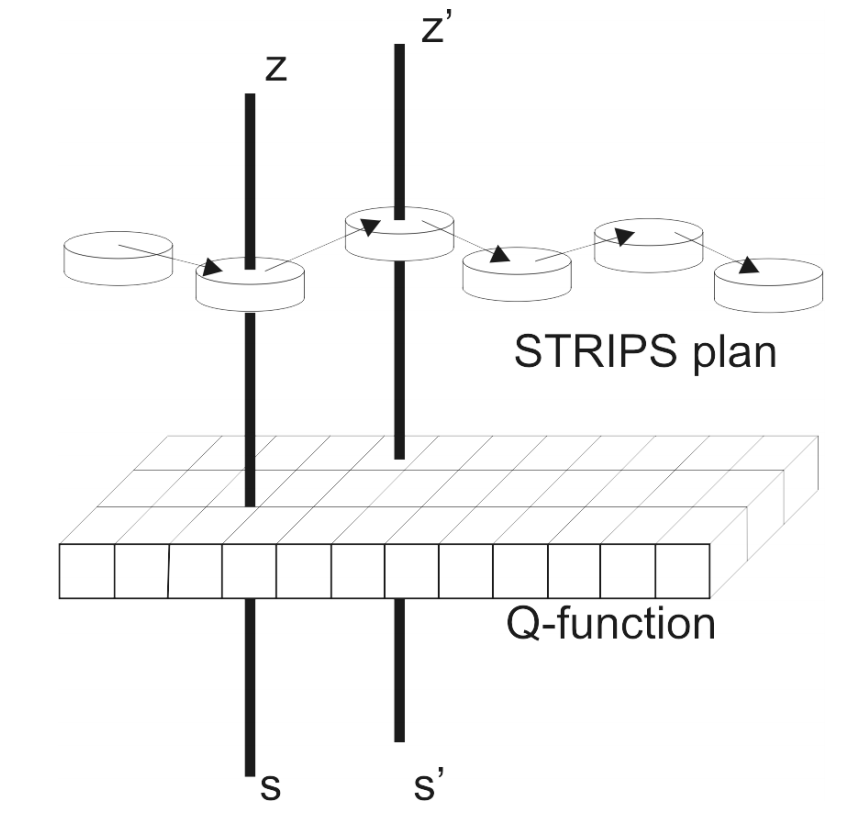
\includegraphics[width = \linewidth]{../article/img/strips.png}
  %\caption{Plan-base reward shaping}
  \label{fig:strips}
\end{figure}

\end{column}

\begin{column}{0.5\linewidth}

\begin{block}{Main idea}
\begin{itemize}
\item Plan: set of subgoals
\item Subgoals: state of the agent\\$\rightarrow$ domain specific
\item To be followed
\item Reward proportional to the distance of the step in the plan
\end{itemize}
\end{block}

\begin{block}{Potential Function}
\begin{itemize}
\item $\phi (s) = \omega * CurrentStepInPlan$
\item $\omega$ : scaling factor
\item $\omega = MaxReward/NumStepsInPlan$
\item Max shaping reward = max domain reward
\end{itemize}
\end{block}

\end{column}

\end{columns}



\end{frame}


\begin{frame}{Multi-Agent Planning}

\begin{block}{Centralized Planning}
\vskip-1em
\begin{columns}[onlytextwidth]

\begin{column}{0.5\textwidth}

\begin{itemize}
\item Generate global plan
\item Decompose it
\item Assign task to multiple agents
\item Divulge plans and goals
\end{itemize}
$\rightarrow$ Joint-plan

\end{column}


\begin{column}{0.5\textwidth}

\begin{figure}[h!]
\centering
  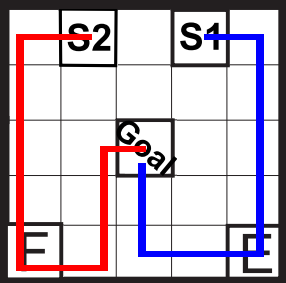
\includegraphics[height=0.35\textheight]{../article/img/joinrExemple.png}
  \label{fig:studycase1}
\end{figure}

\end{column}
\end{columns}

\end{block}


\begin{block}{Decentralized Planning}
\vskip-1em
\begin{columns}[onlytextwidth]

\begin{column}{0.5\textwidth}

\begin{itemize}
\item Each agent set its own plan
\item Do not divulge plans and goals
\end{itemize}
$\rightarrow$ Individual-plan

\end{column}
\begin{column}{0.5\textwidth}

\begin{figure}[h!]
\centering
  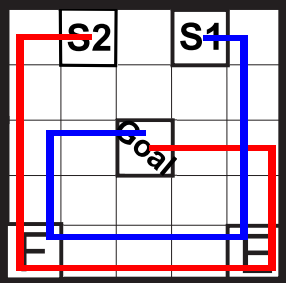
\includegraphics[height=0.35\textheight]{../article/img/individualExemple.png}
  \label{fig:studycase1}
\end{figure}

\end{column}

\end{columns}
\end{block}




\end{frame}

\begin{frame}{Problem}

\begin{columns}[t]
\begin{column}{0.5\linewidth}
\begin{figure}[h!]
\centering
  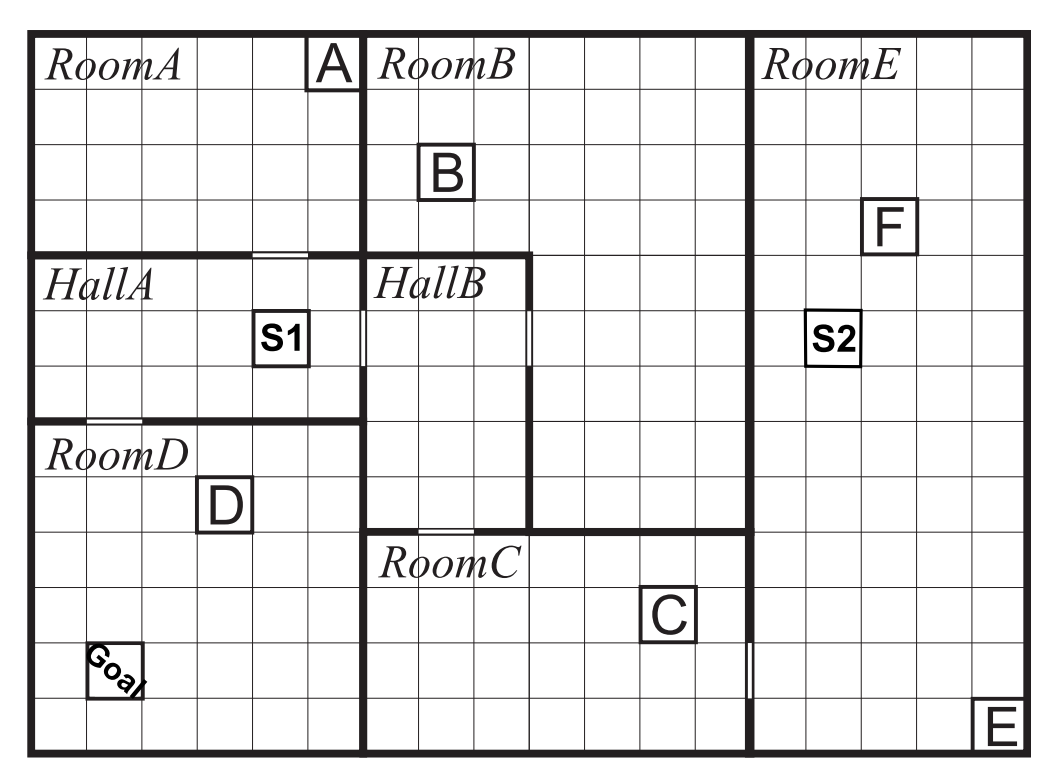
\includegraphics[width=\linewidth]{../article/img/stydyCase.png}
  \caption{Multi-Agent, Flag-Collecting Problem Domain.}
  \label{fig:studycase1}
\end{figure}
\end{column}

\begin{column}{0.5\linewidth}
\begin{block}{Description}
\begin{itemize}
\item Two agents
\item Six flags
\item Seven rooms
\item One goal
\item Reward  $\left\{
\begin{array}{l}
on\ goal =  Flags*100 \\
not\ on\ goal = 0
\end{array}
\right.$
\item Agent knows its position
\item Agent knows the flags it collected
\item Episode : start to goal
\end{itemize}


\end{block}
\end{column}

\end{columns}

\end{frame}
\begin{frame}{Plan Handling}

\begin{columns}
\begin{column}{0.6\linewidth}
\begin{figure}[h!]
\centering
  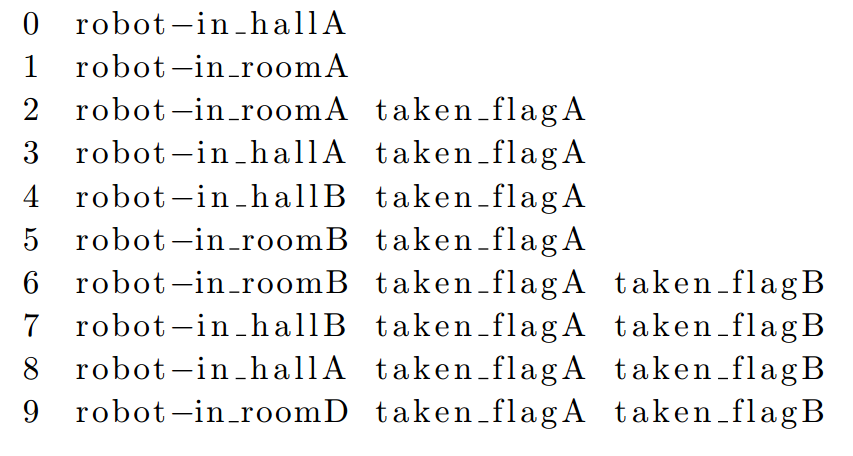
\includegraphics[width = \linewidth]{../article/img/listingFormattedJoinAgent1.png}
  \caption{State based plan}
  \label{fig:plan2}
\end{figure}
\end{column}


\begin{column}{0.4\linewidth}
\begin{figure}[h!]
\centering
  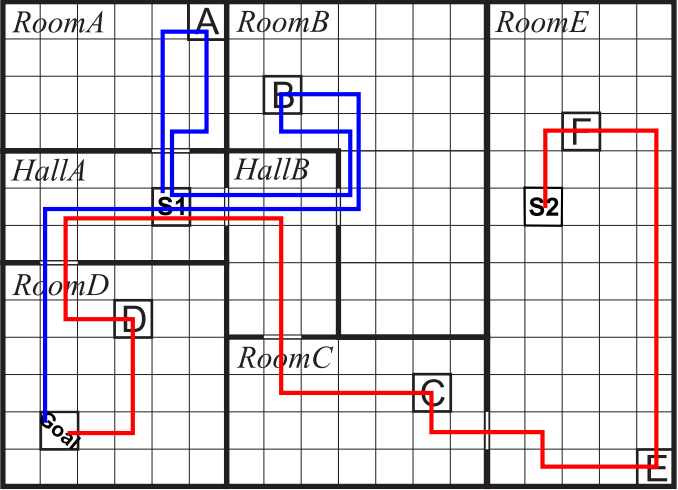
\includegraphics[width = \linewidth]{../article/img/jointCase.png}
  \caption{Joint-plan}
  \label{fig:plan2}
\end{figure}
\end{column}

\end{columns}

\begin{block}{}
\begin{itemize}
\item Action based to state based
\item Each agent has an individual-plan and a joint-plan
\end{itemize}
\end{block}

\end{frame}

\begin{frame}{Heuristics}

\begin{block}{Flag-Based}
\begin{itemize}
\item $\phi (s) =  NumFlagsCollected*\omega$
\item $\omega = MaxReward/MaxFlagsInWorld$
\end{itemize}
\end{block}

\begin{block}{Plan-Based}
\begin{itemize}
\item $\phi (s) =  CurrentStepInPlan*\omega$
\item $\omega = MaxReward/NumStepsInPlan$
\item Not in plan $\rightarrow$ last step in plan
\end{itemize}
\end{block}

\begin{block}{Flag-Based and Plan-Based}
\begin{itemize}
\item $\phi (s) = \omega * (CurrentStepInPlan + NumFlagsCollected)$
\item $\omega = MaxReward/(NumStepsInPlan + NumFlagsInWorld)$
\end{itemize}
\end{block}

\end{frame}


\section{Results and Discussion}

\begin{frame}{Experiments}

\begin{block}{Modus operandi}
\begin{itemize}
\item SARSA($\lambda$)
\item $\epsilon$-Greedy
\item $\alpha = 0.1$
\item $\gamma = 0.99$
\item $\epsilon = 0.1$ 
\item $\lambda = 0.4$
\item Q-values initialized to 0
\item 2000 episodes
\item Average over 30 simulations
\item Discounted total reward over episodes
\item Discounted total reward = $reward*\gamma^{steps}$
\item Value averaged over 100 previous episodes


\end{itemize}
\end{block}

\end{frame}

\begin{frame}{Initial Results}

\begin{columns}

\begin{column}{0.65\linewidth}

\begin{figure}[h!]
  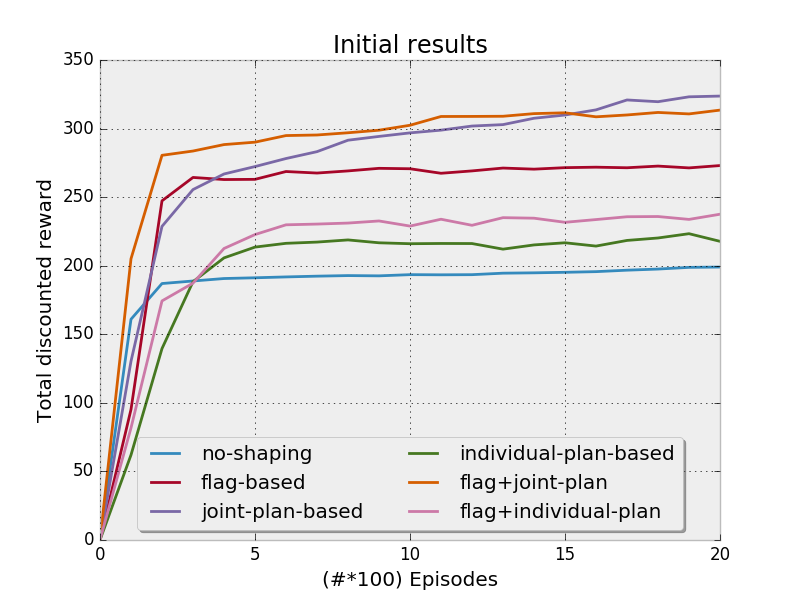
\includegraphics[width = \linewidth]{../article/img/initial.png}
  %\caption{Initial results.}
  \label{fig:results1}
\end{figure}

\end{column}


\begin{column}{0.45\linewidth}

\begin{block}{Analysis}
\begin{itemize}
\item Lower bound : no shaping
\item Upper bound : joint-plan
\item Individual-plan : poor results
\item Flag-based : inefficient path
\item Plan-based and flag-based : add knowledge
\end{itemize}
\end{block}

\end{column}

\end{columns}

\end{frame}

\begin{frame}{Conflicted Knowledge}

\begin{columns}[onlytextwidth]
\begin{column}{0.5\linewidth}

\begin{figure}[h!]
  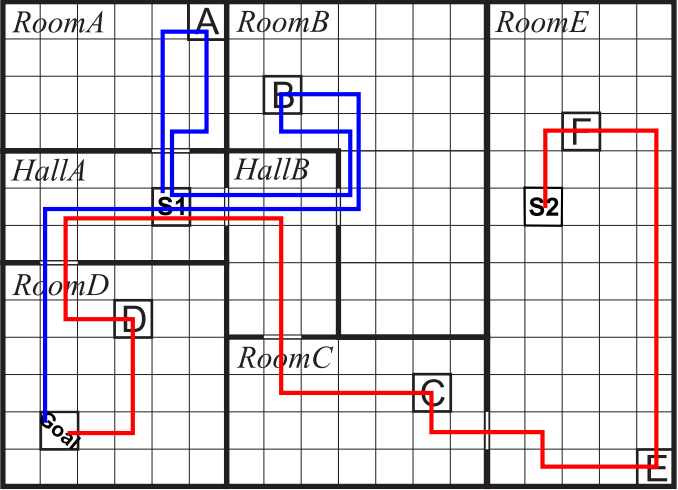
\includegraphics[height=0.4\textheight]{../article/img/jointCase.png}
  %\caption{Behaviours of :}
  \label{fig:behave}
\end{figure}
\end{column}

\begin{column}{0.5\linewidth}

\begin{figure}[h!]
  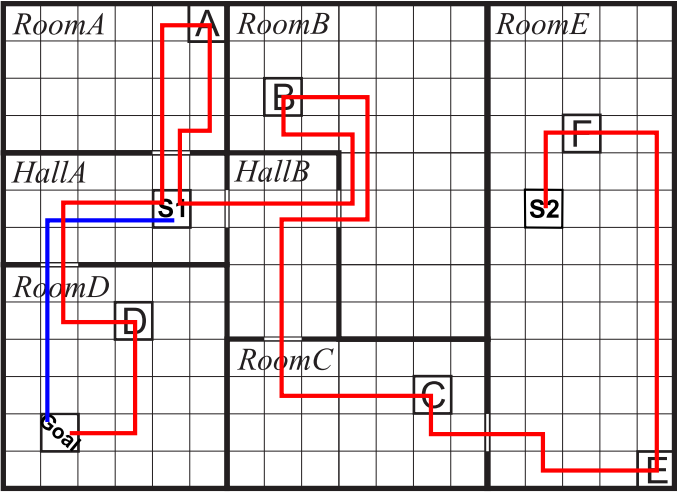
\includegraphics[height=0.4\textheight]{../article/img/individualCase.png}
  %\caption{Behaviours of :}
  \label{fig:behave}
\end{figure}
\end{column}

\end{columns}

\begin{columns}[onlytextwidth]
\begin{column}{0.45\linewidth}

\begin{alertblock}{}
\begin{itemize}
\item Poor behaviour with individual plans
\item Conflict knowledge
\item How to avoid it ?
\item \textbf{Make individual-plan based reward shaping as efficient as the joint-plan one}
\end{itemize}
\end{alertblock}
\end{column}

\begin{column}{0.5\linewidth}
\hfill
\begin{figure}[h!]
  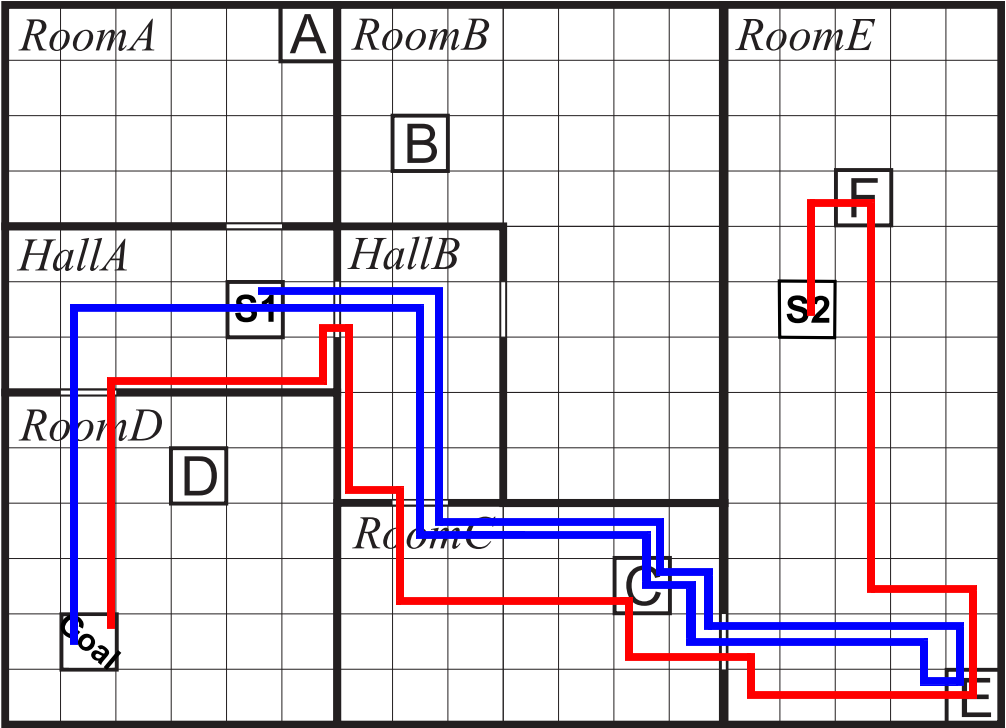
\includegraphics[height=0.4\textheight]{../article/img/conflictCase.png}
  %\caption{Behaviours of :}
  \label{fig:behave}
\end{figure}
\end{column}

\end{columns}

\end{frame}

\begin{frame}{Partial Knowledge}



\begin{columns}
\begin{column}{0.65\linewidth}

\begin{figure}[h!]
  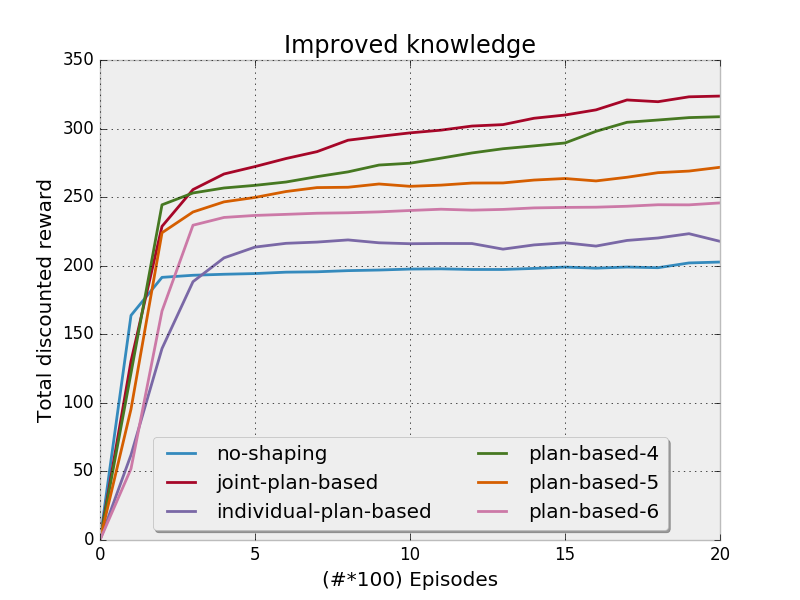
\includegraphics[width=\linewidth]{../article/img/knowledge.png}
  %\caption{Improved knowledge.}
  \label{fig:results2}
\end{figure}

\end{column}

\begin{column}{0.45\linewidth}
\begin{block}{Explanation and Analysis}
\begin{itemize}
\item Delayed conflict
\item Removed conflict
\item Significant improvement
\item Need global knowledge
\end{itemize}
\end{block}
\end{column}

\end{columns}


\end{frame}

\begin{frame}{Improved Cooperation}



\begin{columns}
\begin{column}{0.65\linewidth}


\begin{figure}[h!]
  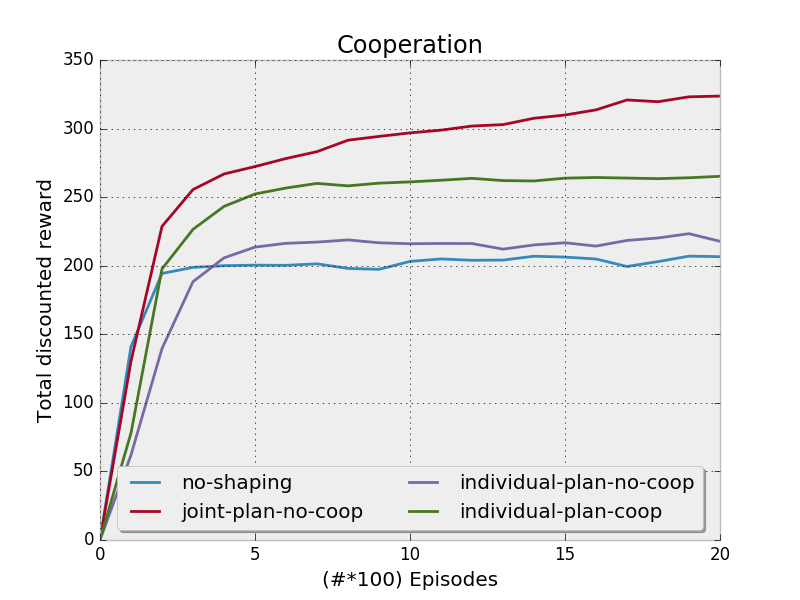
\includegraphics[width=\linewidth]{../article/img/coop.png}
  %\caption{Improved knowledge.}
  \label{fig:results2}
\end{figure}

\end{column}

\begin{column}{0.45\linewidth}

\begin{block}{Explanation and Analysis}
\begin{itemize}
\item Agents share collected flags
\item Minimal communication
\item Clear improvement
\item Does not reach joint-plan
\item Individual-plan remains non optimal
\end{itemize}
\end{block}
\end{column}

\end{columns}

\end{frame}


\section{Conclusion}

\begin{frame}{Conclusion}

\begin{block}{}
\begin{itemize}
\item Knowledge improves results
\item Joint-plan is optimal
\item Individual-plans leads to conflicted knowledge
\item Posterior cooperation is not sufficient to overcome it
\item Transforming the plan to avoid conflict works
$\rightarrow$ Is it possible to automate it ?
\end{itemize}
\end{block}

\end{frame}

\begin{frame}{Other and Future Work}

\begin{block}{Other work}
\begin{itemize}
\item Exploration can overcome conflict knowledge but needs more episodes
\item Abstract-MDP reward shaping
\end{itemize}
\end{block}

\begin{block}{Future Work}
\begin{itemize}
\item Use specific MARL algorithms
\item Modify potential function according to domain
\end{itemize}

\hspace*{.1\linewidth}\begin{minipage}{.8\linewidth}
\begin{center}
\begin{exampleblock}{Knowledge revision}
Interpret conflict knowledge as bad or incomplete knowledge and use knowledge revision\\
$\rightarrow$ Two steps:
\begin{itemize}
\item Implement knowledge revision for multi-agent
\item Experiment it with individual-plans
\end{itemize}
\end{exampleblock}

\end{center}
\end{minipage}
\medskip
\end{block}

\end{frame}


\end{document}